%****************************************************************
% Chapter X
%****************************************************************
\label{chapter-implementation}
\chapter{Implementation}

In this chapter, details of the major implementation are revealed. First, briefly introducing Google VR SDK setup and drawing with OpenGL ES. Then an explanation of the web server design. After that, the creation of 3D virtual scene is highlighted. Finally, the implementation for device movement and object intersection detection are  clarified.

%****************************************************************
\section{Google VR SDK}

The Google VR SDK repository is free and accessible from\href{https://github.com/googlevr/gvr-android-sdk}{\emph{https://github.com/googlevr/gvr-android-sdk}}, where we can get access to any necessary libraries and examples. The SDK libraries locate in the libraries directory of the repository as \emph{.aar} files \cite{google.aar-format.2016}. This project has two dependencies on \code{base} and \code{common} Google VR SDK modules.

%****************************************************************
\section{OpenGL ES}

OpenGL assumes a square coordinate system, by default, happily draws those coordinates onto the screen. However screens can vary in size and shape, that is to say, most screens are typically non-square screen. The illustration below \ref{fig:opengl-coordinates} shows the assumed uniform coordinate system of an OpenGL frame on the left, and how these coordinates map to an exemplary non-square device screen in landscape orientation on the right.

\begin{figure}[H]
\caption[OpenGL coordinate system mapping]{Default OpenGL coordinate system (left) mapped to a typical Android device screen (right) \cite{google.opengles.2016}}
\label{fig:opengl-coordinates}
\centering
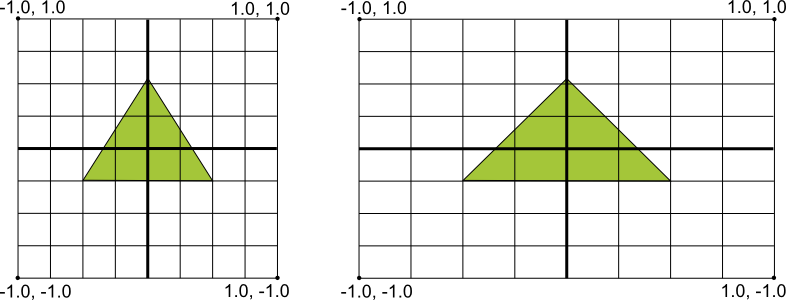
\includegraphics[width=\linewidth]{Figures/opengl-coordinates.png}
\decoRule
\end{figure}

Therefore, OpenGL projection modes and camera views have to be applied to the OpenGL rendering pipeline for coordinates transformation, so the graphic objects have the expected proportions on any display. The projection matrix will recalculate the coordinates of graphics objects, and the camera view matrix will create a transformation that renders objects from a specific eye position.

The implementation is divided into two phases. First, working out the model matrix, view matrix, and perspective matrix in CPU (Android programming in this case). Secondly pass them to GPU for the rest of calculation (OpenGL Shading Language Programming, i.e. GLSL or GLslang), such as explicit projection matrix, coordinates transformation, lighting, or more abstract circular ring \ref{section:ray-pointer}. The GLSL shaders themselves are a set of strings that passed to the hardware driver for compiling within an application using the OpenGL API's entry points \cite{wiki.glsl.2016}.

\begin{table}[H]
\caption{OpenGL compute}
\label{tab:opengl-compute}
\centering
\begin{tabular}{l l l l}
\toprule
\tabhead{What} & \tabhead{How} & \tabhead{Where}\\
\midrule
Model Matrix & translationMx * scaleM * rotationM * identityM(1) & CPU\\
Camera Matrix & Matrix.setLookAtM(positionV, lookAtV, upV) & CPU\\
View Matrix & eye.getEyeView() * cameraM & CPU\\
Perspective Matrix & eye.getPerspective(zNear, zFar) & CPU\\
Projection Matrix & perspectiveM * viewM * modelM & GPU\\
Vertex' & projectionM * vertex & GPU\\
\bottomrule
\end{tabular}
\end{table}

%****************************************************************
\section{Web Server}

See the example below, a simple file server on port \code{8080} to serve a directory on disk "\emph{/tmp}" under an alternate URL path "\emph{/files/}", using \code{StripPrefix} to modify the request URL's path before the \code{FileServer} sees it.

\[
\begin{array}{lr}
\scriptsize{\code{http.Handle("/files/", http.StripPrefix("/files", http.FileServer(http.Dir("./tmp"))))}}\\
\scriptsize{\code{http.ListenAndServe(":8080"), nil)}}\\
\end{array}
\]

For RESTful APIs setup, I introduce a free framework Go-Json-Rest \cite{antoine.go-json-rest.2016}, it is a thin layer designed by KISS principle (Keep it simple, stupid) and on top of native net/http package that helps building RESTful JSON APIs even easier.

%****************************************************************
\subsection{Assets}

The file server processes the requests and delivers the result (the particular file) in a standard web format back to the client. Table \ref{tab:assets-structure} indicates the folder structure served by the server.

\begin{table}[H]
\caption{Assets structure}
\label{tab:assets-structure}
\centering
\begin{tabular}{l l l}
\toprule
\tabhead{Path} & \tabhead{Usage}\\
\midrule
\textbackslash assets & Root\\
\textbackslash assets\textbackslash static.zip & The compressed Patch (see \ref{section:patch}) \\
\textbackslash assets\textbackslash static\textbackslash kml & KML storage (see \ref{section:kml})\\
\textbackslash assets\textbackslash static\textbackslash layer & KML storage (see \ref{section:scene})\\
\textbackslash assets\textbackslash static\textbackslash model & Extra model storage (see \ref{section:obj-model})\\
\textbackslash assets\textbackslash static\textbackslash resource & Resource (eg. images) storage\\
\bottomrule
\end{tabular}
\end{table}

%****************************************************************
\subsection{Patch}
\label{section:patch}

A Path is for the server to guarantee the latest data (if any) will be pushed to each client (Android smartphone). It server as a compressed ZIP file, and it contains one or more files that require client to update. Patch validation is happening whenever the app starts. First, the client sent requests for the patch file "\emph{http://xxx.xxx.xxx.xxx:8080/assets/static.zip}" from the file server. Before actual download the file, take the \code{lastModifiedTime} data of remote Patch from HTTP response headers, and compare it with the other \code{lastModifiedTime} data of local's Patch file. Only when the local's Patch is out of date, the client continues to download the remote Patch file and replacing any existing local files. For a special scenario when the app was just installed in the first time launch, also the network is disconnected. A built-in default Patch that included in the APK (Android app binary) will be uncompressed to avoid no available data. Diagram \ref{fig:patch-check} shows the simplified process.

\begin{figure}[H]
\caption{Patch check}
\label{fig:patch-check}
\centering
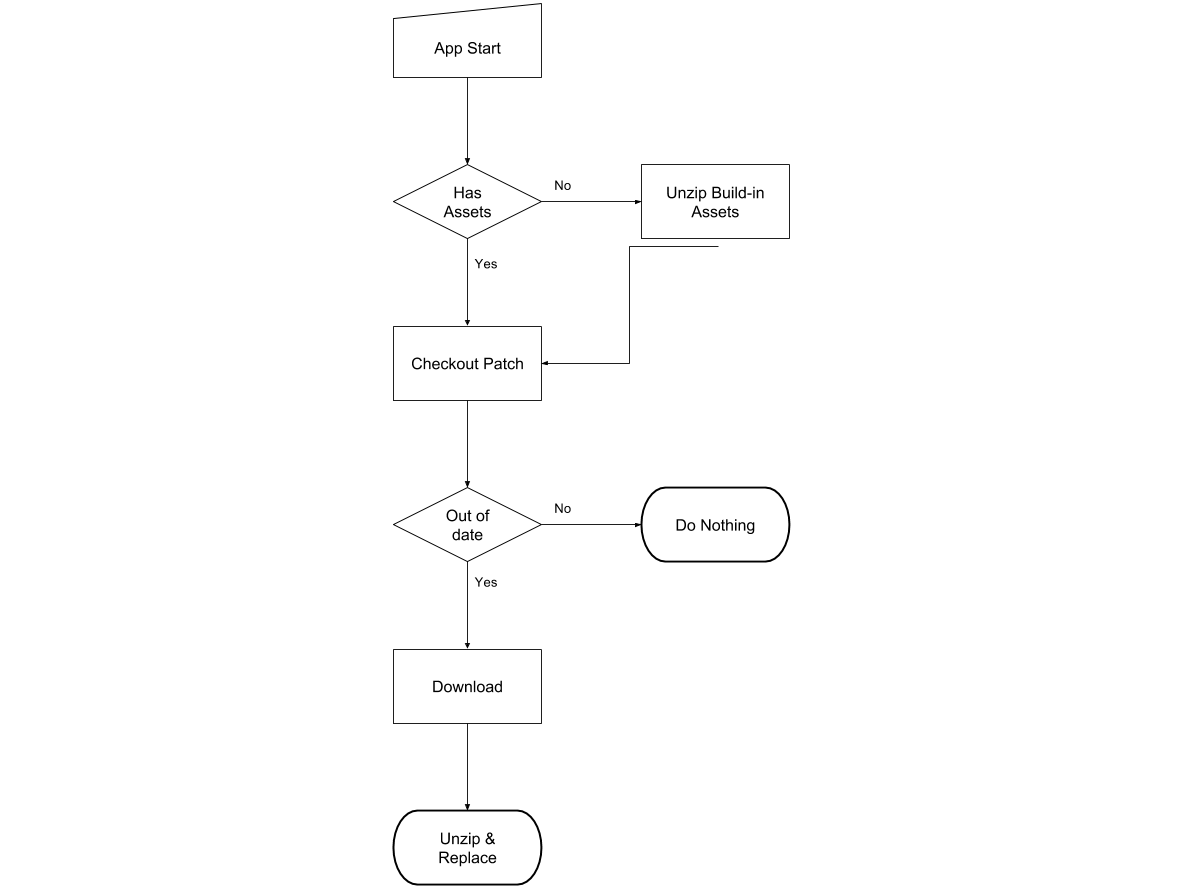
\includegraphics[width=\linewidth]{Figures/patch-check.png}
\decoRule
\end{figure}

%****************************************************************
\section{Scene}
\label{section:scene}

The Keyhole Markup Language (KML) is contributed to the application as the geographic visualization markup language. KML files from folder "\emph{/assets/static/layer} are visible to the user, and each KML file represents an individual 3D scene which contains any necessary geographic data related to the topic.

As you can see from table \ref{tab:assets-structure}, there are two assets folders contains KML files - "\emph{/assets/static/layer}" and "\emph{/assets/static/kml}". These files are literally the same, but existing in different concepts for achieving the purpose of categorizing. By making use of \code{Networklink} facility, an individual KML file can contains one or more other KML files by given URLs. Therefore, folder "\emph{/assets/static/layer}" intends to be the scene topic (KML file) storage that visible and selectable to the user, and any inside topic could include one or more topics that exist in folder "\emph{/assets/static/kml}".

It has many advantages to dividing the space with certain patterns during the space creation. Such as, runtime graphical analysis and optimization, intersection and collision detection.

%****************************************************************
\subsection{Geographic Visualization Markup Language}
\label{section:kml}

There are only some of KML features from KML schema \ref{fig:kml-schema} are be used in this application. They are \code{Container}, \code{Style}, \code{Placemark}, and \code{NetworkLink}. The KML parser I am using is not coded from scratch, and it is based on the open-source library \code{android-maps-utils} \cite{google.code-kml.2016} but with certain modification and extension: getting rid of \code{GoogleMap} dependency; extending \code{NetworkLink} facility support that was one of the unsupported features in the library.

\begin{figure}[H]
\caption{kML parser simple}
\label{fig:kml-parser-simple}
\centering
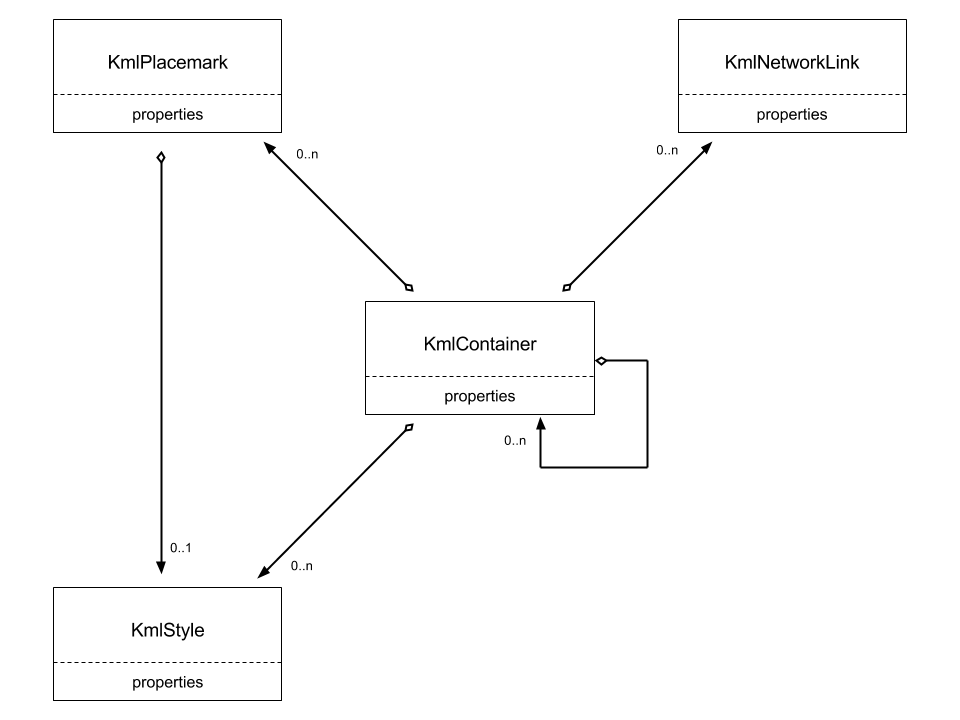
\includegraphics[width=\linewidth]{Figures/kml-parser-simple.png}
\decoRule
\end{figure}

%****************************************************************
\subsection{Space Partition} 
\label{section:space-partition}

Space partition often used for optimizing collision detection algorithms among polygonal models. These algorithms are often expensive operations and can significantly slow FPS down. Although there is no collision detection in this application yet, there is an intersection detection between the ray tracing (see \ref{section:ray-pointer}) and other objects. Space partition is contributed to reducing the ray-object intersection test load by skipping objects that locate far away from current ray tracing area. It avoids doing an $n^2$ times intersection detection on all objects.

A axis-aligned Octree is implemented for the space partition \ref{fig:octree-split}. It has a predefined constant positive integer to decide whether or not a new partitioning should happen - a minimum number of objects allowed exist in the same cell. This number is important for the purpose of reducing intersection detections. I have taken $5$, object complexity and cell complexity need to be considered.

\begin{description}
	\setlength{\parskip}{0pt}
	\item[$\bullet$ Object Complexity] \code{Plackmarker} is doing ray-sphere detection (see \ref{section:ray-sphere})
	\item[$\bullet$ Cell Complexity] Cell is doing ray-box detection (see \ref{section:ray-box})
\end{description}

If the number is positive infinity - whole space seen as a cell and no further space partition is required, this is not reduce anything but also increase to $n + 1$ times of detections ($n$ times for ray-object, $1$ times for ray-cell). If the number is $1$ - each cell only contains one object, this also not reduces the number of detection times, but increase to at least $2\,n$ times. Since the ray-box detection action is much cheaper then ray-sphere's, an appropriate value can eventually reduce the overall intersection detections.

\begin{figure}[H]
\caption{Octree split}
\label{fig:octree-split}
\centering
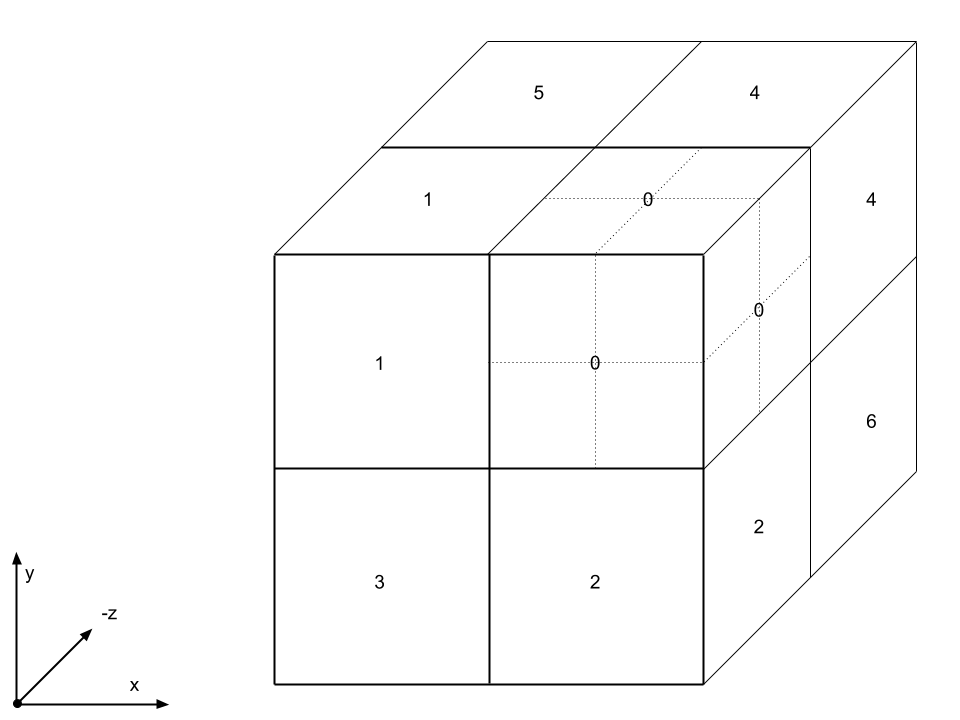
\includegraphics[width=\linewidth]{Figures/octree-split.png}
\decoRule
\end{figure}

See diagram \ref{fig:octree-split}, the parent cell has eight indexes indicate the different relative position inside the parent cell. These indexes are important for the next time of division, where the objects in parent cell need to be relinked to a new cell. On the other words, a new object will be linked to the parent cell only if the existed objects is less than the predefined constant value. If not, the parent cell will be spatially divided into eight cells. Then, the existing objects will be unlinked from the parent cell and relink to a new cell.

The integer index is not chosen randomly. It is defined by its geometric meaning - three boolean value that indicates the three axis-relative delta value. Table \ref{tab:octree-octant} gives the relationship between the index and three boolean values.

The three delta values of any position $P$ in a cell with known center $O$ are:

\[
\begin{array}{lr}
\begin{aligned}
dx &= P_x - O_x\\
dy &= P_y - O_y\\
dz &= P_z - O_z\\
\end{aligned}
\end{array}
\]

The relationship between the index and three boolean values as follow:

\begin{table}[H]
\caption{Octree octant}
\label{tab:octree-octant}
\centering
\begin{tabular}{l l l l}
\toprule
\tabhead{Binary Index} & \tabhead{Octant} & \tabhead{Geometric Meaning}\\
\midrule
0x00000000 & T,\;T,\;T & dx > 0, dy > 0, dz > 0\\
0x00000001 & F,\;T,\;T & dx < 0, dy > 0, dz > 0\\
0x00000010 & T,\;F,\;T & dx > 0, dy < 0, dz > 0\\
0x00000011 & F,\;F,\;T & dx < 0, dy < 0, dz > 0\\
0x00000100 & T,\;T,\;F & dx > 0, dy > 0, dz < 0\\
0x00000101 & F,\;T,\;F & dx < 0, dy > 0, dz < 0\\
0x00000110 & T,\;F,\;F & dx > 0, dy < 0, dz > 0\\
0x00000111 & F,\;F,\;F & dx < 0, dy < 0, dz < 0\\
\bottomrule
\end{tabular}
\end{table}

$\therefore$ The transformation from known index to three boolean values (Octant):

\[
\code{octant[] = (index \& 1, index \& 2, index \& 4)}
\]

The transformation from known Octant to index:

\[
\begin{array}{lr}
\begin{aligned}
\code{For Each oction[i]:}&\\
&\code{index |= (1 < < i)}\\
\end{aligned}
\end{array}
\]

%****************************************************************
\section{Earth}

UV Sphere often used in the situation where requires a very smooth, symmetrical surface. In this application, the Earth model is created as the UV sphere. Similar to latitude and longitude lines of the earth, it uses rings and segments (near the poles, the vertical segments converge on the poles). Therefore, the UV texturing for 2D Earth image mapping to the 3D sphere's surface can be conveniently calculated during its vertex creation process.

\begin{figure}[H]
\caption{UV sphere mapping}
\label{fig:uv-sphere-mapping}
\centering
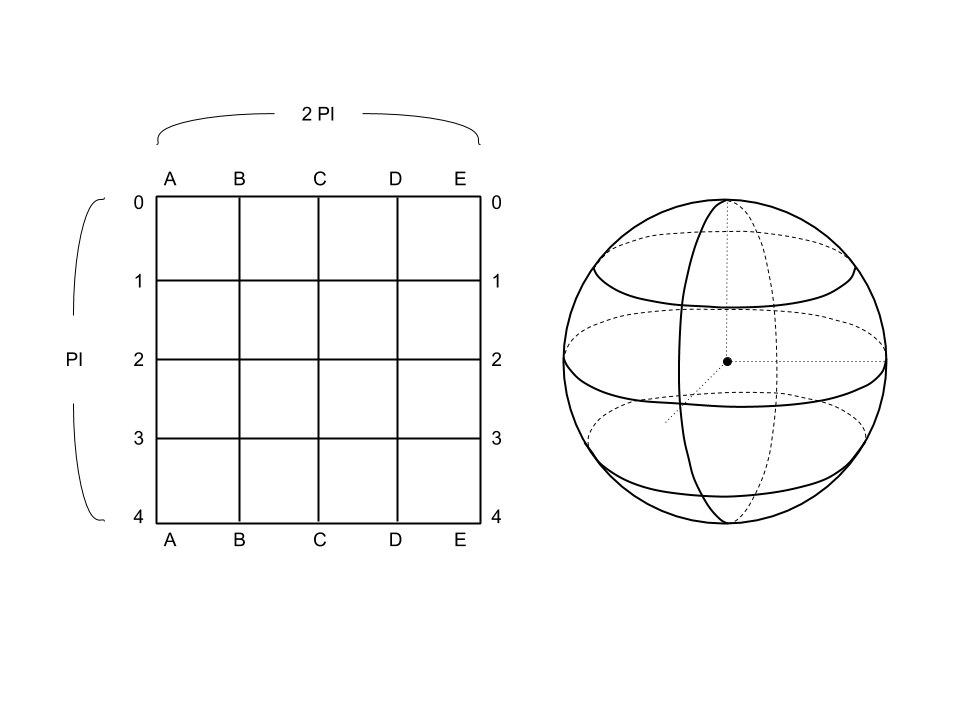
\includegraphics[width=\linewidth]{Figures/uv-sphere-mapping.png}
\decoRule
\end{figure}

The diagram \ref{fig:uv-sphere-mapping} illustrates the mapping from 2D plane to 3D UV sphere's surface which has $5$ rings and $4$ segments. As we can seen, vertex $A0$, $A1$, $A2$, $A3$, $A4$ and $E0$, $E1$, $E2$, $E3$, $E4$ are duplicated; vertex $A0$, $B0$, $C0$, $D0$, $E0$ converge together in the pole, as well as $A4$, $B4$, $C4$, $D4$, $E4$. Also, in the UV sphere, each ring spans $2\,\pi$ radians, but each segment only spans $\pi$ radians.

The total vertex count for a UV sphere is:

\begin{equation}
\label{equ:uv-sphere-vertices}
\code{VerticesCount} = \code{RingsCount} \times \code{SegmentsCount}
\end{equation}

\begin{figure}[H]
\caption{UV sphere vertex}
\label{fig:uv-sphere-vertex}
\centering
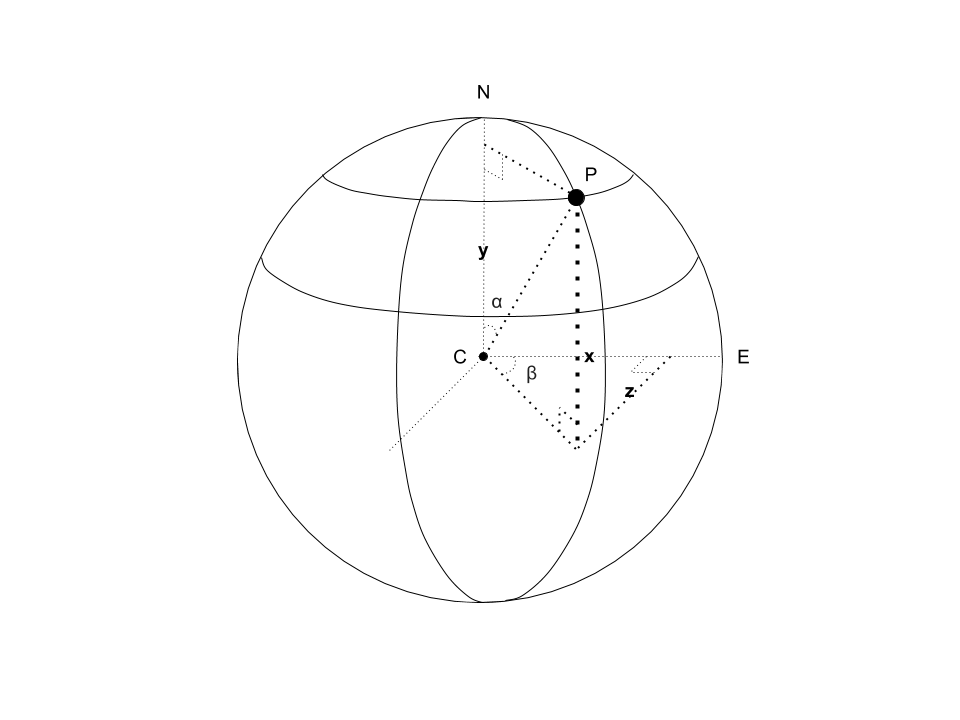
\includegraphics[width=\linewidth]{Figures/uv-sphere-vertex.png}
\decoRule
\end{figure}

If a vertex $P$ on the UV sphere belongs to ring $r$ and segment $s$:

\[
\begin{array}{lr}
v = r \times  \dfrac{1}{\code{RingsCount} - 1}\\\\
u = s \times  \dfrac{1}{\code{SegmentsCount} - 1}\\\\
\measuredangle \alpha = v \times \pi\\
\measuredangle \beta = u \times 2\,\pi\\
\end{array}
\]

$\therefore$ The vertex P (x,\;y,\;z) can be calculated:
\[
\begin{array}{lr}
x = (\sin(\alpha) \times radius) \times \cos(\beta)\\
y = \cos(\alpha) \times radius\\
z =  (\sin(\alpha) \times radius) \times \sin(\beta)\\
\end{array}
\]

The UV texturing (x,\;y) mapping for vertex $P$ is:

\[
\begin{array}{lr}
x = u\\
y = v\\
\end{array}
\]

%****************************************************************
\section{Placemarker}

Generation of vertices for placemarker is a recursion process of subdividing icosphere. Figure \ref{fig:icosahedron-rectangles} shows that the initial vertices of an icosahedron are the corners of three orthogonal rectangles.

\begin{figure}[H]
\caption[Icosahedron rectangles]{Icosahedron rectangles \cite{wiki.icosahedron-rectangles.2006}}
\label{fig:icosahedron-rectangles}
\centering
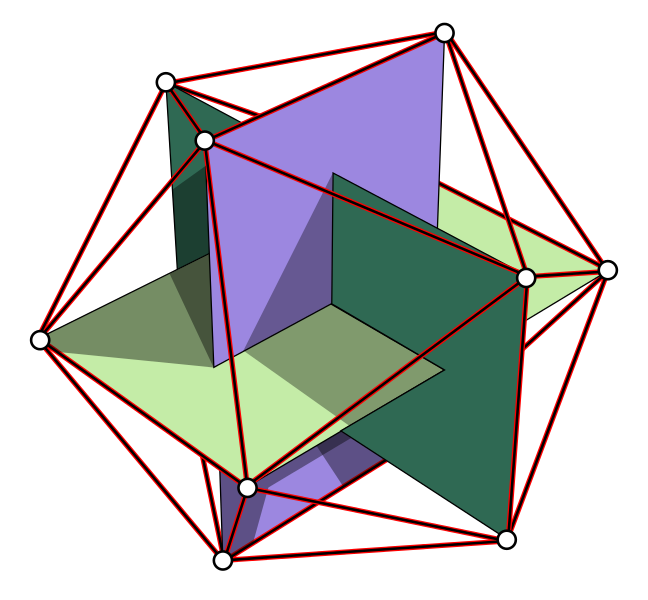
\includegraphics[width=\linewidth]{Figures/icosahedron-rectangles.png}
\decoRule
\end{figure}

Rounding icosphere by subdividing a face to an arbitrary level of resolution. One face can be subdivided into four by connecting each edge's midpoint.

\begin{figure}[H]
\caption{Icosphere subdivide}
\label{fig:icosphere-subdivide}
\centering
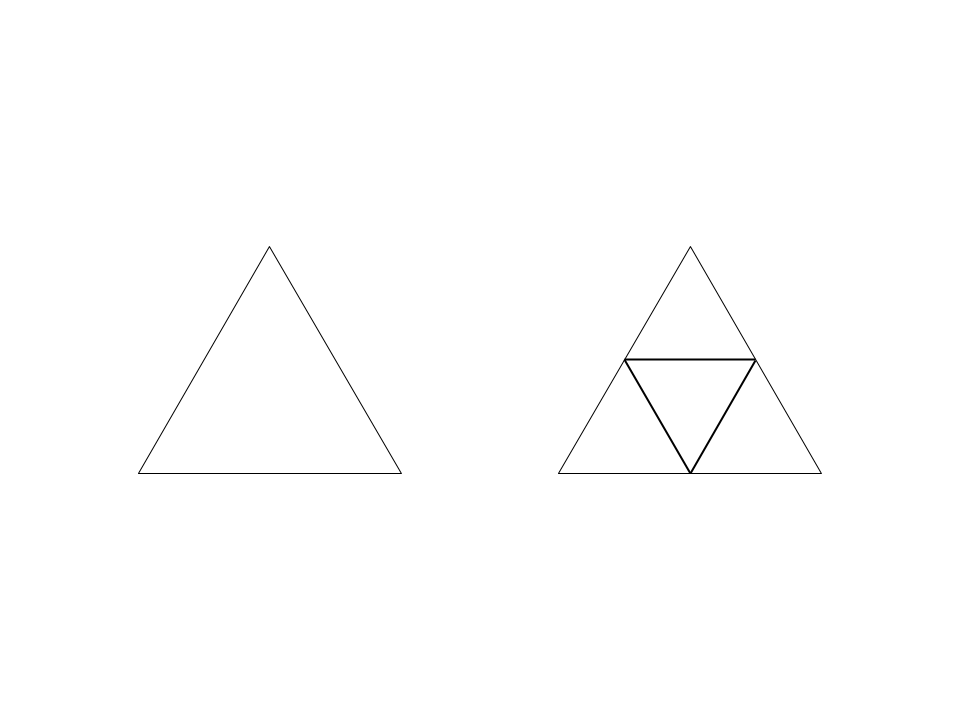
\includegraphics[width=\linewidth]{Figures/icosphere-subdivide.png}
\decoRule
\end{figure}

Then, push edge's midpoints to the surface of the sphere.

\begin{figure}[H]
\caption{Icosphere refinement}
\label{fig:icosphere-refinement}
\centering
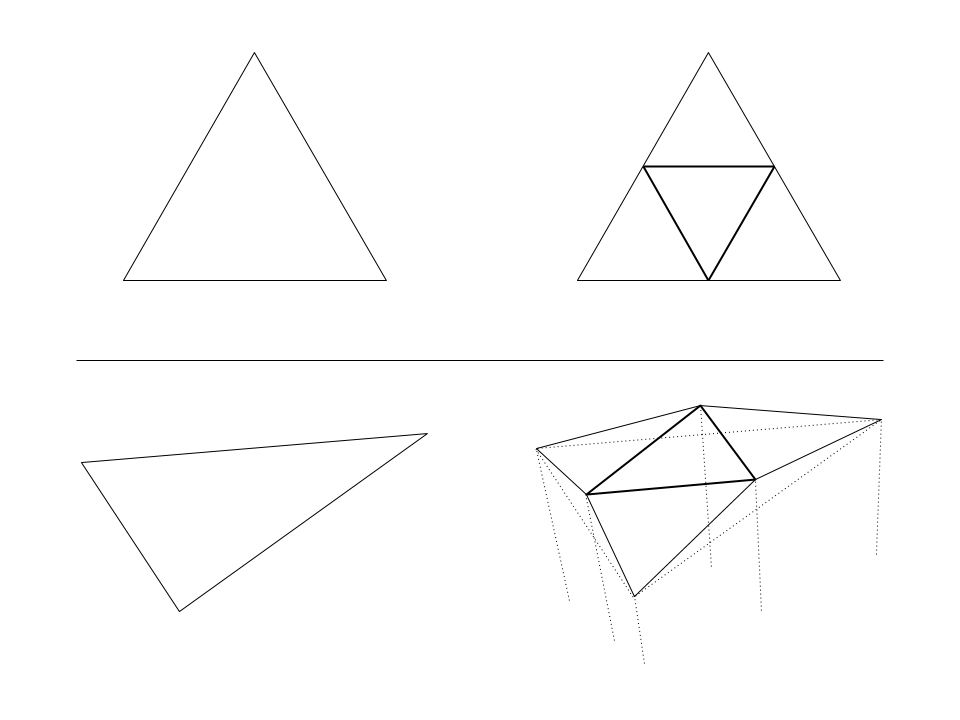
\includegraphics[width=\linewidth]{Figures/icosphere-refinement.png}
\decoRule
\end{figure}

\begin{table}[H]
\caption{Rounding Icosphere}
\label{tab:rounding-icosphere}
\centering
\begin{tabular}{l l l l}
\toprule
\tabhead{Recursion Level} & \tabhead{Vertex Count} & \tabhead{Face Count} & \tabhead{Edge Count}\\
\midrule
0 & 12 & 20 & 30\\
1 & 42 & 80 & 120\\
2 & 162 & 320 & 480\\
3 & 642 & 1280 & 1920\\
\bottomrule
\end{tabular}
\end{table}

%****************************************************************
\subsection{Geographic Coordinate System}

A geographic coordinate system is a coordinate system that enables every location on the Earth to be specified by a set of numbers or letters, or symbols \cite{wiki.geographic-coordinate-system.2016}. A common geodetic-mapping coordinates are latitude, longitude, and altitude (LLA), which also is the raw location data read from KML.

We introduce ECEF ("earth-centered, earth-fixed") coordinate system for converting LLA coordinates to position coordinates. According to, the z-axis is pointing towards the north but it does not coincide exactly with the instantaneous earth rotational axis. The x-axis intersects the sphere of the earth at $0$ latitude and $0$ longitude \cite{wiki.ecef.2016}.

\begin{figure}[H]
\caption[ECEF]{Earth-centered, earth-fixed \cite{wiki.ecef.2016}}
\label{fig:ecef}
\centering
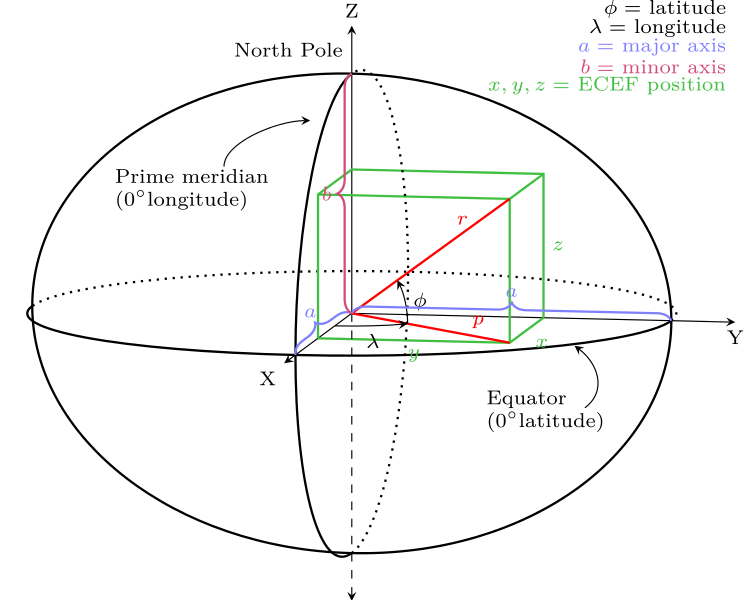
\includegraphics[width=\linewidth]{Figures/ecef.png}
\decoRule
\end{figure}

The ECEF coordinates are expressed in a reference system that is related to mapping representations. Because the earth has a complex shape, a simple, yet accurate, method to approximate the earth’s shape is required. The use of a reference ellipsoid allows for the conversion between ECEF and LLA \cite{ublox.datum.1999}.

A reference ellipsoid can be described by a series of parameters that define its shape and which include a semi-major axis ($a$), a semi-minor axis ($b$), its first eccentricity ($e_1$) and its second eccentricity ($e_2$) as shown in Table \ref{tab:wgs-84-parameters}.

\begin{table}[H]
\caption{WGS 84 parameters}
\label{tab:wgs-84-parameters}
\centering
\begin{tabular}{l l l}
\toprule
\tabhead{Parameter} & \tabhead{Notation} & \tabhead{Value}\\
\midrule
Reciprocal of flattening & $1 / f$ & 298.257\,223\,563\\
Semi-major axis & $a$ & 6\,378\,137\,m\\
Semi-minor axis & $b$ & $a\,(1 - f)$\\
First eccentricity squared & $e_1^2$ & $1 - b^2 / a^2 = 2\,f - f^2$\\
Second eccentricity squared & $e_2^2$ & $a^2 / b^2 - 1 = f\,(2 - f) / (1 - f)^2$\\
\bottomrule
\end{tabular}
\end{table}

\begin{figure}[H]
\caption{Ellipsoid parameters}
\label{fig:ellipsoid-parameters}
\centering
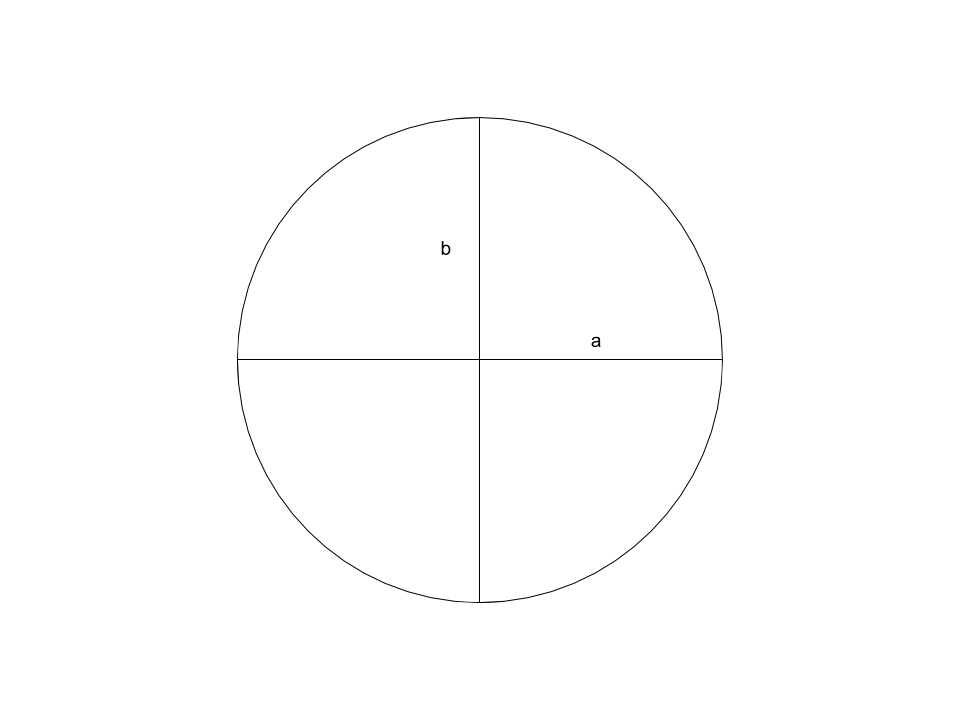
\includegraphics[width=\linewidth]{Figures/ellipsoid-parameters.png}
\decoRule
\end{figure}

The conversion from LLA to ECEF is shown below.

\begin{figure}[H]
\caption{LLA to ECEF}
\label{fig:lla2ecef}
\centering
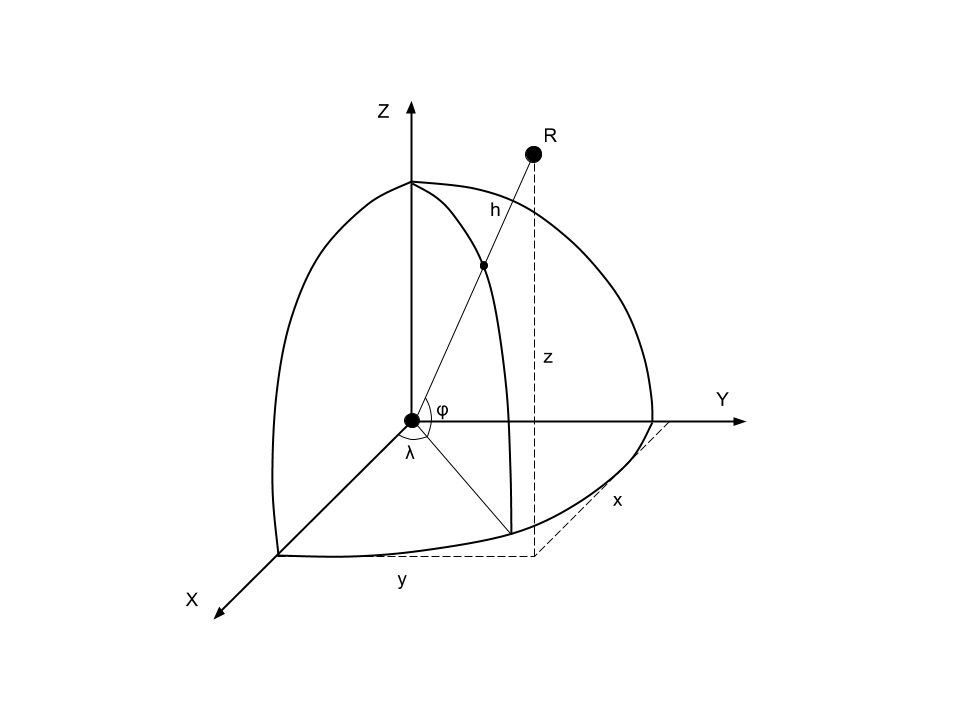
\includegraphics[width=\linewidth]{Figures/lla2ecef.png}
\decoRule
\end{figure}

\[
\begin{array}{lr}
\begin{aligned}
x &= (N + h)\,\cos(\varphi)\,\cos(\lambda)\\
y &= (N + h)\,\cos(\varphi)\,\sin(\lambda)\\
z &= (\dfrac{b^2}{a^2}\,N + h)\,\sin(\varphi)\\
\end{aligned}
\end{array}
\]

Where

\[
\begin{array}{lr}
\begin{aligned}
\varphi &= \text{latitude}\\
\lambda &= \text{longitude}\\
h &= \text{height above ellipsoid (meters)}\\
N &= \text{Radius of Curvature (meters), defined as:}\\
&= \dfrac{a}{\sqrt{1 - e^2\,\sin(\varphi)^2}}\\
\end{aligned}
\end{array}
\]

At last, for this project usage, where high accuracy is not required, $a$ equals to $b$. And also the ECEF coordinate system is y-east, z-north (up), and x points to $0$ latitude and $0$ longitude, but for project specific, we still need to convert ECEF to x-east, y-north (up), and x points to $0$ latitude and $180$ longitude.

%****************************************************************
\subsection{Description}

Description of placemarker requires an appropriate analysis for display. The raw data of description is a set of characters that could be a normal text, an image URL, a URL returns different type of content, or maybe just some meaningless characters.

Although the implementation of analysis in this project did not cover every situation, but it is flexible and extendable for more functionality.

\begin{figure}[H]
\caption{Description analysis}
\label{fig:description-analysis}
\centering
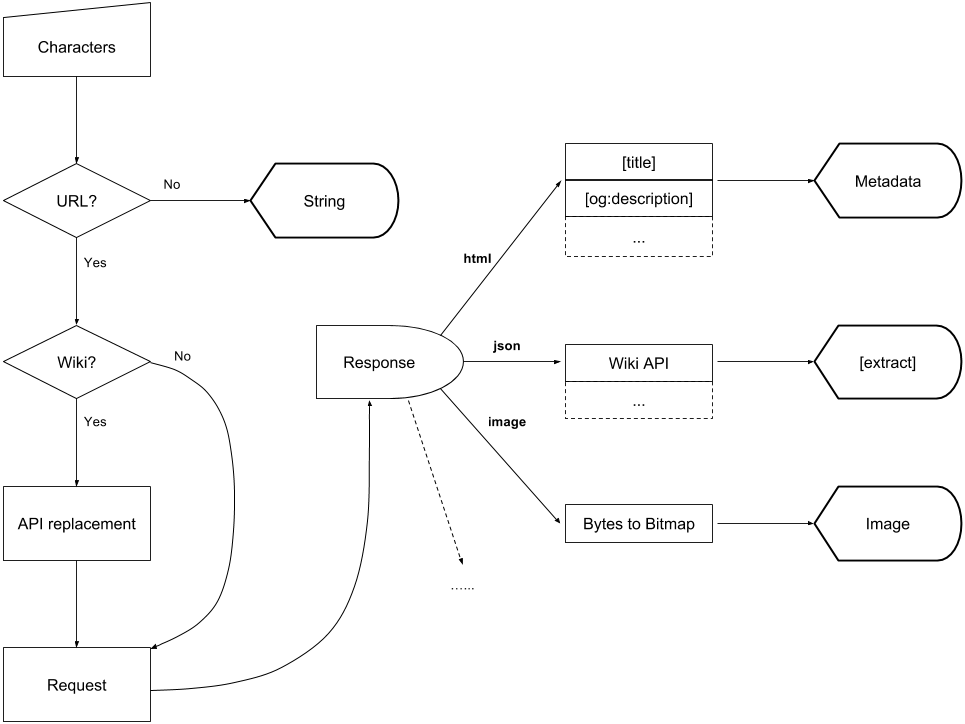
\includegraphics[width=\linewidth]{Figures/description-analysis.png}
\decoRule
\end{figure}

In order to get an extracted content from a Wikipedia page, we can transform the URL to a Wiki-API based open-search URL \cite{wiki.api.2016}, which will return a json format raw data that we can easily get what we need from different json tags.

\[
\begin{array}{lr}
\begin{aligned}
\text{Replace}\;&\code{.wikipedia.org/wiki/}\\
\text{To}\;&\code{.wikipedia.org/w/api.php?}APIs\\
\end{aligned}
\end{array}
\]

Where $APIs$ is:

\[
\begin{array}{lr}
\begin{aligned}
\code{format=json}&\\
&\code{\&action=query}\\
&\code{\&redirects=1}\\
&\code{\&prop=extracts}\\
&\code{\&exintro=}\\
&\code{\&explaintext=}\\
&\code{\&indexpageids=}\\
&\code{\&titles=}\\
\end{aligned}
\end{array}
\]

For $html$ parser, we introduced jsoup (it is a Java library for working with real-world HTML \cite{joup.2016}), to get the basic information we need, such as $title$, and some other metadata. In this project, I am also using $og:description$ (one of the open graph meta tags \cite{ogp.2014}) from the HTML source if it exist.

%****************************************************************
\subsection{Extra Model}
\label{section:obj-model}

A simple and common OBJ format model can be loaded as an extra model for the placemarker. OBJ model can be generated by Blender \cite{blender.2016}. A simple OBJ parser is created only support v (vertex indices), vn (vertex normals), fv (face vertex), fvn (face vertex normals), and MTL syntax is ignored \cite{shen.obj-parser.2011}.

%****************************************************************
\section{Ray Pointer}
\label{section:ray-pointer}

%****************************************************************
\section{Information Display}

A textfield is a rectangle vertex based renderable component to display text on a flat plane. Since it is a GL scene, the actual text will be drawn as a texture. By a constant width and native \code{android.text.StaticLayout} support, the height of the texture can be calculated. 

A menu contains multi-textfield can be seen as an empty textfield based which texture is fill-full a pure background color, and several textfields are laid out on the top of it with a certain vertical dimension.

A head rotation matrix (quaternion matrix \cite{jvv.quaternions.2013}) is required for locating object in front of camera \cite{mathworks.quaternion-rotation.2016}.

%****************************************************************
\section{Camera Movement}

In general, there are two sensors can be useful to manage camera movement: ACCELEROMETER (API level 3), LINEAR\_ACCELERATION (API level 9) and STEP\_DETECTOR (API level 19). 

LINEAR\_ACCELERATION is same as ACCELERATION which measures the acceleration force in meter per second repeatedly, except linear acceleration sensor is a synthetic sensor with gravity filtered out. 

\[
\begin{array}{lr}
Linear Acceleration = Accelerometer Data - Gravity\\
v = \int a\,dt\\
x = \int v\,dt\\
\end{array}
\]

First of all, we take the accelerometer data and remove gravity that is called gravity compensation, whatever is left is linear movement. Then we have to integrate it one to get velocity, integrated again to get the position, which is called double integral. Now if the first integral creates drift, double integrals are really nasty that they create horrible drift. Because of this noise, using acceleration data it isn't so accurate, it is really hard to do any kind of linear movement \cite{google.sensor-fusion.2010}.

On the other hand, use step counter from STEP\_DETECTOR, and pedometer algorithm for pedestrian navigation, that in fact works very well for this project.

\[
\begin{array}{lr}
p_1 = p_0 + v_0 \times dt\\
v_1 = v_0 + a \times dt\\
\end{array}
\]

The accuracy of this depends on how precision we can get for changing velocity. Considering that velocity is made of 3-axis directions, the current heading direction is required for a correct velocity calculation. Since the frame life cycle is implemented based on \cite{google.vr-sdk.2016}, which provide the heading direction in each frame callback. So I collect everything I need from the last frame to new frame and update both velocity and position for each new frame.

First of all, damping is required. I reduce velocity by a percentage. It is simply for avoiding that camera taking too long to stop. Damping by percentage can stable and stop the camera in a certain of time that won't be affected by the current camera speed. 

Secondly, a constant value in head forwarding direction is been used as a pulse for each step. Because a step is happening instantaneously which implies $a\,dt$ made by each step is actually can be replaced by a constant value.

\begin{figure}[H]
\caption{Camera movement}
\label{fig:camera-movement}
\centering
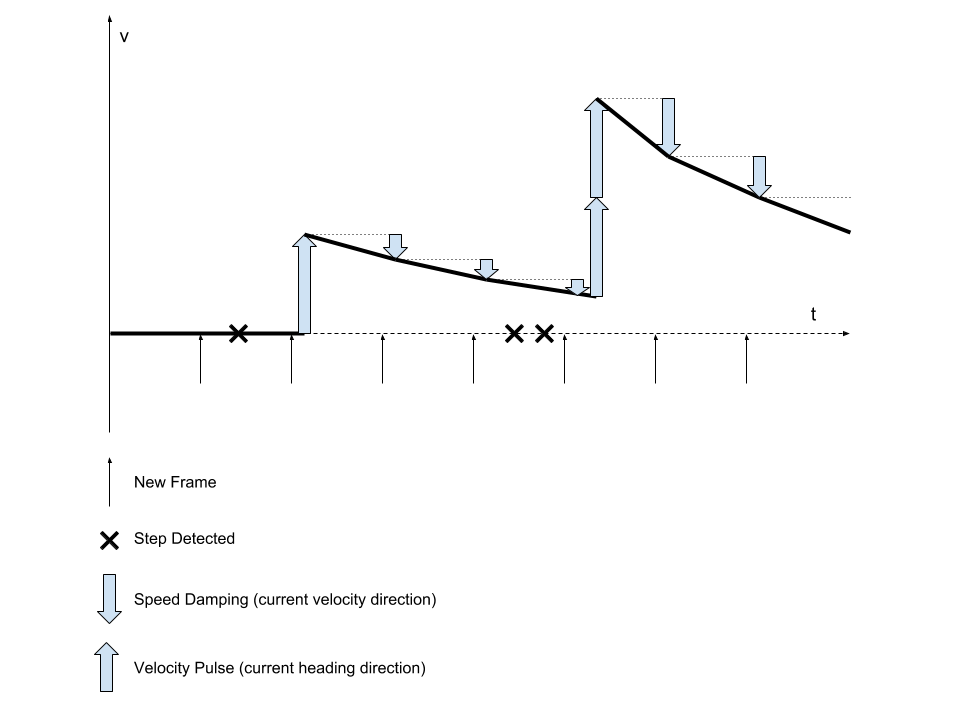
\includegraphics[width=\linewidth]{Figures/camera-movement.png}
\decoRule
\end{figure}

For each new frame:

\[
\begin{array}{lr}
\begin{aligned}
\overrightarrow{V_0} &= \overrightarrow{V_0} \cdot Damping\\
\overrightarrow{P_1} &= \overrightarrow{P_0} + \overrightarrow{V_0} \cdot dt\\
\overrightarrow{V_1} &= \overrightarrow{V_0} + \overrightarrow{Forwarding} \cdot Pulse \cdot Steps\\
Damping &\in [0,\enspace1]\\
Pulse &\in [0,\enspace \infty)\\
\end{aligned}
\end{array}
\]

%****************************************************************
\section{Ray Intersection}

Detect collisions between ray and models are the key to allowing user selecting objects in the VR would, which is one of the important experience for user interaction.

A ray can be describe in a equation with known ray start position \emph{$\overrightarrow{R_0}$} and ray direction \emph{$\overrightarrow{R_d}$}.

\begin{equation}
\label{equ:ray-t}
\overrightarrow{R(t)} = \overrightarrow{R_0} + \overrightarrow{R_d} \cdot t
\end{equation}

%****************************************************************
\subsection{Ray-Sphere}
\label{section:ray-sphere}

\begin{figure}[H]
\caption{Ray-Sphere intersection}
\label{fig:ray-sphere}
\centering
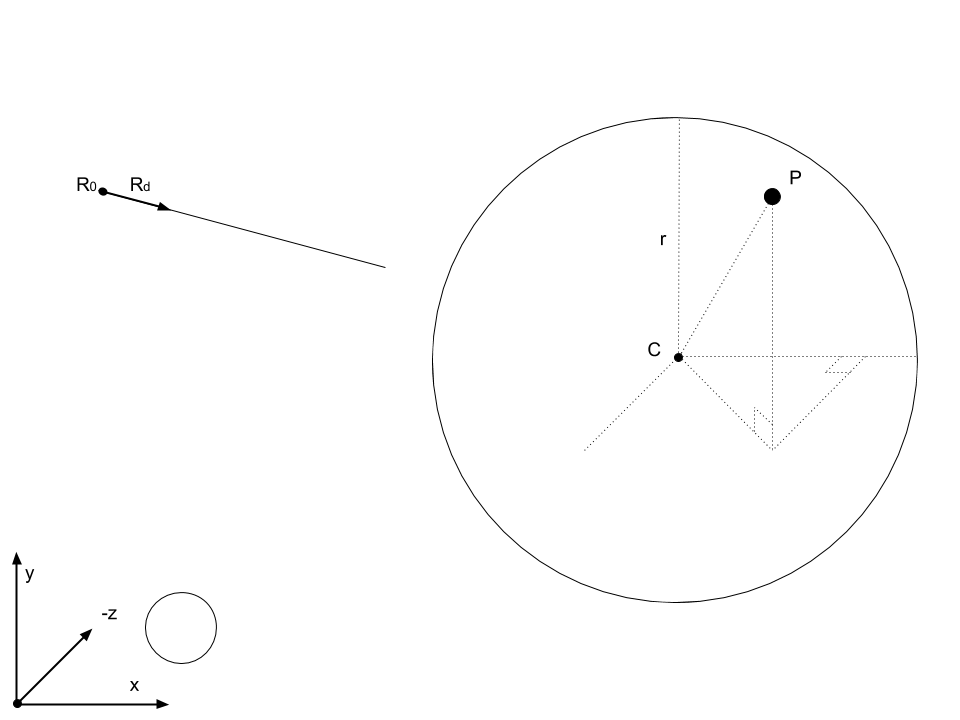
\includegraphics[width=\linewidth]{Figures/ray-sphere-intersection.png}
\decoRule
\end{figure}

A point \emph{P} on the surface of sphere should match the equation:

\begin{equation}
\label{equ:sphere-surface}
(x_p - x_c)^2 + (y_p - y_c)^2 + (z_p - z_c)^2 = r^2
\end{equation}

If the ray intersects with the sphere at any position\;\emph{P} must match the equation \ref{equ:ray-t} and \ref{equ:sphere-surface}. Therefore the solution of \emph{t} in the cointegrate equation implies whether or not the ray will intersect with the sphere:

\[
\begin{aligned}
(x_{R_0} + x_{R_d} \cdot t - x_c)^2 &+ (y_{R_0} + y_{R_d} \cdot t - y_c)^2 + (z_{R_0} + z_{R_d} \cdot t - z_c)^2 = r^2\\
&\vdots\\
x_{R_d}^2\,t^2 &+ (2\,x_{R_d}\,(x_{R_0} - x_c))\,t + (x_{R_0}^2 - 2\,x_{R_0}\,x_c + x_c^2)\\
+\;y_{R_d}^2\,t^2 &+ (2\,y_{R_d}\,(y_{R_0} - y_c))\,t + (y_{R_0}^2 - 2\,y_{R_0}\,y_c + y_c^2)\\
+\;z_{R_d}^2\,t^2 &+ (2\,z_{R_d}\,(z_{R_0} - z_c))\,t + (z_{R_0}^2 - 2\,z_{R_0}\,z_c + z_c^2) = r^2\\
\end{aligned}
\]

It can be seen as a quadratic formula:

\begin{equation}
\label{equ:sphere-surface-quadratic-formula}
a\,t^2 + b\,t + c = 0
\end{equation}

At this point, we are able to solved the \emph{t}:

\[
t =
\begin{cases}
\dfrac{-b \pm \sqrt{b^2 - 4\,a\,c}}{2\,a} & \text{if }\;b^2 - 4\,a\,c > 0\\
\dfrac{-b}{2\,a} & \text{if }\; b^2 - 4\,a\,c = 0\\
\varnothing & \text{if }\; b^2 - 4\,a\,c < 0\\
\end{cases}
\]

Then, I take a further step to get rid of formula complexity.

$\because$ Equation \ref{equ:sphere-surface},\,\ref{equ:sphere-surface-quadratic-formula}
\[
\begin{array}{lr}
a = x_{R_d}^2 + y_{R_d}^2 + z_{R_d}^2\\
b = 2\,(x_{R_d}\,(x_{R_0} - x_c) + y_{R_d}\,(y_{R_0} - y_c) + z_{R_d}\,(z_{R_0} - z_c))\\
c = (x_{R_0} - x_c)^2 + (y_{R_0} - y_c)^2 + (z_{R_0} - z_c)^2 - r^2\\
\end{array}
\]

$\And$
\[
\begin{array}{lr}
\begin{aligned}
\norm{\overrightarrow{R_d}} &= \sqrt{x_{R_d}^2 + y_{R_d}^2 + z_{R_d}^2} = 1\\
\overrightarrow{V_{c\_R_0}} &= \overrightarrow{R_0} - \overrightarrow{C} = \overrightarrow{(x_{R_0} - x_c,\enspace y_{R_0} - y_c,\enspace z_{R_0} - z_c)}\\
\end{aligned}
\end{array}
\]

$\therefore$
\[
\begin{array}{lr}
a =1\\
b = 2 \cdot \overrightarrow{R_d} \cdot \overrightarrow{V_{c\_R_0}}\\
c = \overrightarrow{V_{c\_R_0}} \cdot \overrightarrow{V_{c\_R_0}} \cdot r^2\\
\end{array}
\]

$\because$ The formula for \emph{t} can also be optimized
\[
\begin{array}{lr}
\dfrac{-b \pm \sqrt{b^2 - 4\,a\,c}}{2\,a} = -\alpha \pm \sqrt{\beta}\\
\alpha = \dfrac{1}{2}\,b\\
\beta = \alpha^2 - c\\
\end{array}
\]

$\therefore$ The final solution for \emph{t}
\[
t =
\begin{cases}
 -\alpha \pm \sqrt{\beta} & \text{if }\;\beta > 0\\
-\alpha & \text{if }\;\beta = 0\\
\varnothing & \text{if }\;\beta < 0\\
\end{cases}
\]

And the collision position for each \emph{t} is:

\[
\overrightarrow{P} = \overrightarrow{R_0} + \overrightarrow{R_d} \cdot t
\]

%****************************************************************
\subsection{Ray-Plane}

\begin{figure}[H]
\caption{Ray-Plane intersection}
\label{fig:ray-plane}
\centering
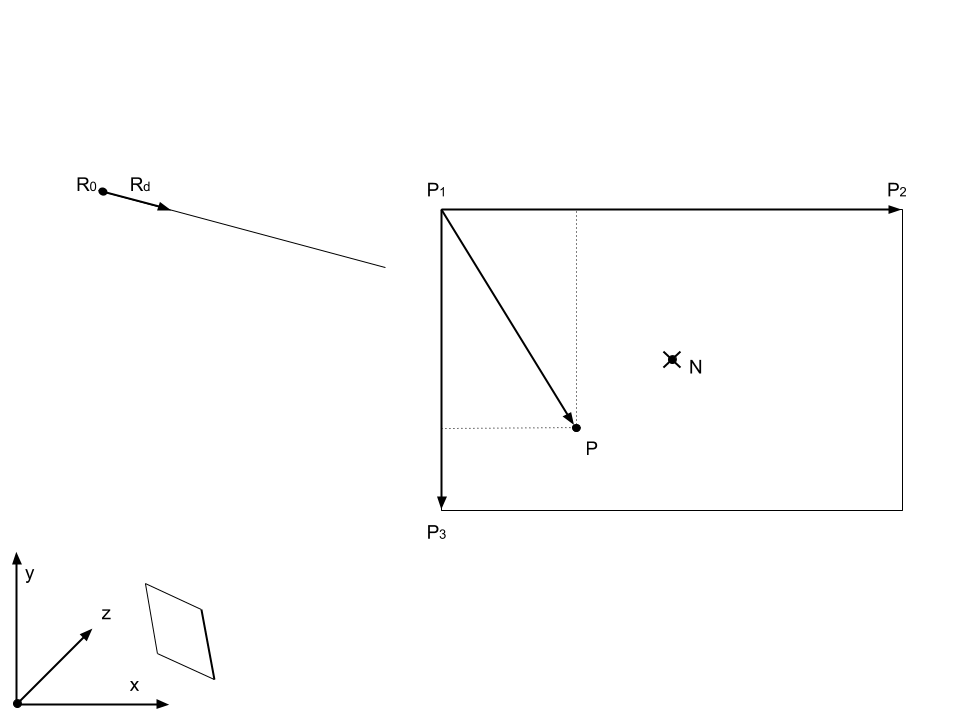
\includegraphics[width=\linewidth]{Figures/ray-plane-intersection.png}
\decoRule
\end{figure}

If a point \emph{P} on the plane and also belongs to the ray, we have quadric equation:

\begin{equation}
\label{equ:ray-plane-intersection}
\begin{array}{lr}
(\overrightarrow{P} - \overrightarrow{P_1}) \cdot \overrightarrow{N} = 0\\
\overrightarrow{P} = \overrightarrow{R_0} + \overrightarrow{R_d} \cdot t\\
\end{array}
\end{equation}

Solution for the \emph{t} is:

\[
t =
\begin{cases}
\dfrac{-\overrightarrow{N} \cdot (\overrightarrow{R_0} - \overrightarrow{P_1})}{\overrightarrow{N} \cdot \overrightarrow{R_d}} & \text{if }\;\overrightarrow{N} \cdot \overrightarrow{R_d} \nsim 0\\
\varnothing & \text{if }\;\overrightarrow{N} \cdot \overrightarrow{R_d} \sim 0\\
\end{cases}
\]

At last, we have to verify if the collision is inside of the quadrangle by putting \emph{t} back to \ref{equ:ray-plane-intersection}, \cite{user3146587.ray-plane.2014} the \emph{t} is valid only if:

\[
\begin{array}{lr}
\mu = \sqrt{(\overrightarrow{P} - \overrightarrow{P_1}) \cdot (\overrightarrow{P_2} - \overrightarrow{P_1}))} \in [0,\enspace\norm{\overrightarrow{P_2} - \overrightarrow{P_1}}]\\
\nu = \sqrt{(\overrightarrow{P} - \overrightarrow{P_1}) \cdot (\overrightarrow{P_3} - \overrightarrow{P_1}))} \in [0,\enspace\norm{\overrightarrow{P_3} - \overrightarrow{P_1}}]\\
\end{array}
\]

%****************************************************************
\subsection{Ray-Box}
\label{section:ray-box}
% \cite{scratchapixel.ray-plane-3d}
% \cite{williams.ray-box.2005}

There is an octree implementation \ref{section:space-partition} in the VR 3D world that separates the 3D world to invisible 3D boxes that each box contains a certain number of other models. It is to avoid unnecessary ray-object collision detection. In this section, I am going to first explain Ray-Box-2D collision detection \cite{tavian.ray-box-2d.2011}, then derive out Ray-Box-3D intersection.

%****************************************************************
\subsubsection{Ray-Box 2D}

\begin{figure}[H]
\caption{Ray-Box 2D intersection}
\label{fig:ray-box-2d}
\centering
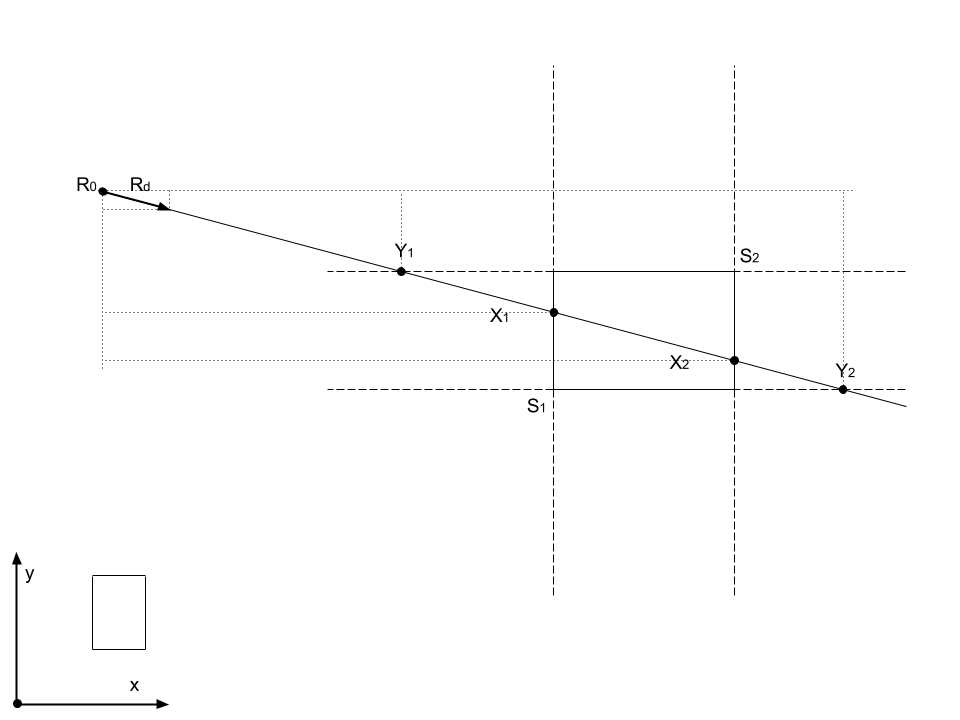
\includegraphics[width=\linewidth]{Figures/ray-box-2d-intersection.png}
\decoRule
\end{figure}

$\because$ Known $R_0$,\enspace$R_d$,\enspace$P_1$,\enspace$P_2$
\begin{multicols}{2}
\noindent
\[
X_1 =
\begin{cases}
x_{P_1} - x_{R_0} & \text{if }\;x_{R_d} > 0\\
x_{P_2} - x_{R_0} & \text{if }\;x_{R_d} < 0\\
\end{cases}
\]
\[
X_2 =
\begin{cases}
x_{P_2} - x_{R_0} & \text{if }\;x_{R_d} > 0\\
x_{P_1} - x_{R_0} & \text{if }\;x_{R_d} < 0\\
\end{cases}
\]
\[
\begin{array}{lr}
t_{X_1} = \dfrac{X_1}{x_{R_d}}\\
t_{X_2} = \dfrac{X_2}{x_{R_d}}\\
\end{array}
\]
\columnbreak
\[
Y_1 =
\begin{cases}
y_{P_1} - y_{R_0} & \text{if }\;y_{R_d} > 0\\
y_{P_2} - y_{R_0} & \text{if }\;y_{R_d} < 0\\
\end{cases}
\]
\[
Y_2 =
\begin{cases}
y_{P_2} - y_{R_0} & \text{if }\;y_{R_d} > 0\\
y_{P_1} - y_{R_0} & \text{if }\;y_{R_d} < 0\\
\end{cases}
\]
\[
\begin{array}{lr}
t_{Y_1} = \dfrac{Y_1}{y_{R_d}}\\
t_{Y_2} = \dfrac{Y_2}{y_{R_d}}\\
\end{array}
\]
\end{multicols}

$\And$ When collision happens, we have formula:
\[
\begin{array}{lr}
\begin{aligned}
t_{X_1} &< t_{X_2}\\
t_{Y_1} &< t_{Y_2}\\
\end{aligned}
\end{array}
\]

$\therefore$ Which is
\begin{equation}
\label{equ:ray-box-2d-intersection}
max(t_{X_1},\enspace t_{Y_1}) < min(t_{X_2},\enspace t_{Y_2})
\end{equation}

%****************************************************************
\subsubsection{Ray-Box 3D}

\begin{figure}[H]
\caption{Ray-Box 3D intersection}
\label{fig:ray-box-3d}
\centering
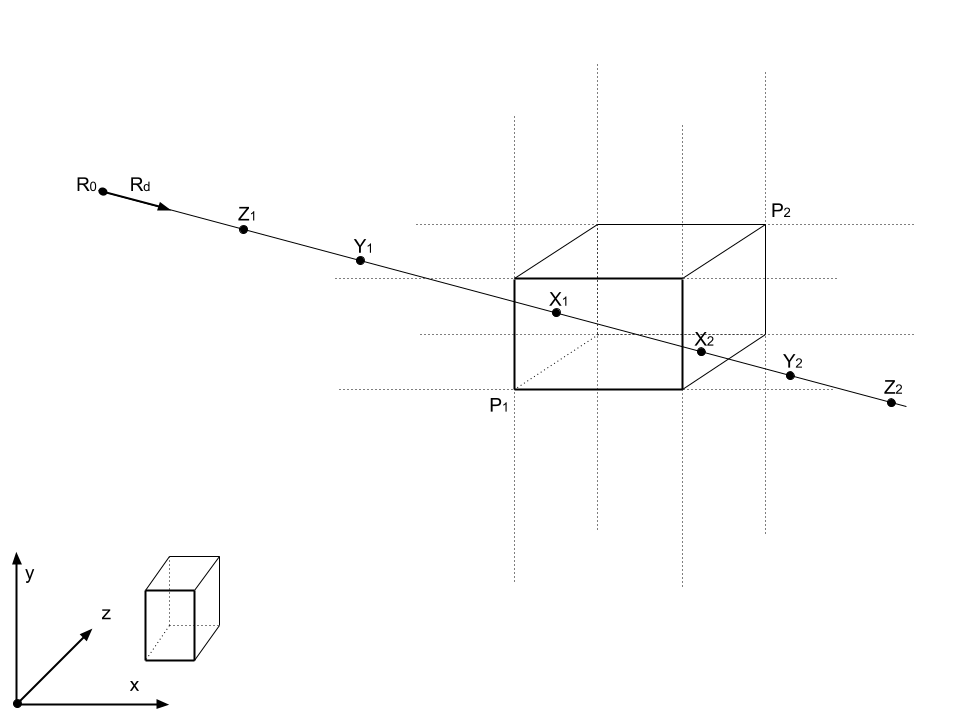
\includegraphics[width=\linewidth]{Figures/ray-box-3d-intersection.png}
\decoRule
\end{figure}

$\because$ Known $R_0$,\enspace$R_d$,\enspace$P_1$,\enspace$P_2$
\begin{multicols}{2}
\noindent
\[
X_1 =
\begin{cases}
x_{P_1} - x_{R_0} & \text{if }\;x_{R_d} > 0\\
x_{P_2} - x_{R_0} & \text{if }\;x_{R_d} < 0\\
\end{cases}
\]
\[
X_2 =
\begin{cases}
x_{P_2} - x_{R_0} & \text{if }\;x_{R_d} > 0\\
x_{P_1} - x_{R_0} & \text{if }\;x_{R_d} < 0\\
\end{cases}
\]
\[
\begin{array}{lr}
t_{X_1} = \dfrac{X_1}{x_{R_d}}\\
t_{X_2} = \dfrac{X_2}{x_{R_d}}\\
\end{array}
\]
\columnbreak
\[
Y_1 =
\begin{cases}
y_{P_1} - y_{R_0} & \text{if }\;y_{R_d} > 0\\
y_{P_2} - y_{R_0} & \text{if }\;y_{R_d} < 0\\
\end{cases}
\]
\[
Y_2 =
\begin{cases}
y_{P_2} - y_{R_0} & \text{if }\;y_{R_d} > 0\\
y_{P_1} - y_{R_0} & \text{if }\;y_{R_d} < 0\\
\end{cases}
\]
\[
\begin{array}{lr}
t_{Y_1} = \dfrac{Y_1}{y_{R_d}}\\
t_{Y_2} = \dfrac{Y_2}{y_{R_d}}\\
\end{array}
\]
\end{multicols}
\begin{multicols}{2}
\noindent
\[
Z_1 =
\begin{cases}
z_{P_1} - z_{R_0} & \text{if }\;z_{R_d} > 0\\
z_{P_2} - z_{R_0} & \text{if }\;z_{R_d} < 0\\
\end{cases}
\]
\[
Z_2 =
\begin{cases}
z_{P_2} - z_{R_0} & \text{if }\;z_{R_d} > 0\\
z_{P_1} - z_{R_0} & \text{if }\;z_{R_d} < 0\\
\end{cases}
\]
\[
\begin{array}{lr}
t_{Z_1} = \dfrac{Z_1}{z_{R_d}}\\
t_{Z_2} = \dfrac{Z_2}{z_{R_d}}\\
\end{array}
\]
\columnbreak
\[
\]
\end{multicols}

$\And$ When collision happens, we have formula:
\[
\left\{
\begin{array}{lr}
\begin{aligned}
t_{X_1} &< t_{X_2}\\
t_{Y_1} &< t_{Y_2}\\
t_{Z_1} &< t_{Z_2}\\
\end{aligned}
\end{array}
\right.
\]

$\therefore$ Which is
\begin{equation}
\label{equ:ray-box-3d-intersection}
max(t_{X_1},\enspace t_{Y_1},\enspace t_{Z_1}) < min(t_{X_2},\enspace t_{Y_2},\enspace t_{Z_2})
\end{equation}

%****************************************************************
